\chapter{Bouncing Rays Through Moving Scenes}\label{ch:Intersection}

To bounce a ray through a scene, checks need to be performed to know which objects it intersects with and thus bounces off of.
These checks are usually done by modelling objects using an equation that describes whether a point is on the object surface or not,
then injecting the ray's function into that equation and resolving.
With static objects, this check is trivial:
The only parameter to resolve for is the intersection time \(t\), and said parameter only occurs in the ray function,
usually making for a first-degree polynomial function.
\newline
As an example, a surface \(S\) can be modelled using a point \(P_1\) on it as well as its normal \(n\).
Then, to tell if any point \(p\) is on \(S\), the vector from \(P_1\) to \(p\) can be compared to \(n\).
If they're orthogonal to each other (thus their dot product is 0), \(p\) is on \(S\):

\begin{equation}\label{StaticSurface}
    (p - P_1) \cdot n = 0
\end{equation}

For a polygon defined by its corner points \(P_{1}\) to \(P_{n}\), the same equation can be used,
with the difference that \(n\) needs to be determined from a set of at least three of the points.
The cross product of two vectors is always orthogonal to both vectors, so using points \(P_{1}\) through \(P_{3}\),
\(n\) can be determined as

\begin{equation}\label{PolygonNormal}
    n = (P_{2} - P_{1}) \times (P_{3} - P_{1})
\end{equation}

Additionally, a polygon needs to further check whether \(p\) is actually inside the bounds defined by its corners.
For triangles, this can be done using barycentric coordinates.
\newline
Barycentric coordinates describe a point on a triangle (or another simplex) by separating a triangle into three parts,
each with the given point and two corners of the triangle as its vertices.
Each coordinate then describes the relative size of that triangle with respect to the full triangle.
% TODO barycentric coords image
\newline
Thus, each point inside the triangle can be described by coordinates \((\alpha, \beta, \gamma)\),
with \(0 \le \alpha \le 1\), \(0 \le \beta \le 1\), \(0 \le \gamma \le 1\) and \(\alpha + \beta + \gamma = 1\).
If these conditions do not apply to \(p\), it is outside the triangle.
\newline
The naive way to calculate barycentric coordinates would be to calculate the areas of \(P_1P_2p\), \(P_1P_3p\), \(P_2P_3p\) and
divide them by the area of \(P_1P_2P_3\)~\cite{SM09}:
\begin{verbatim}
    normal = cross((p3 - p1), (p2 - p1));
    p1p2p = dot(normal, cross((p1 - p), (p2 - p)));
    p1p3p = dot(normal, cross((p3 - p), (p1 - p)));
    p2p3p = dot(normal, cross((p2 - p), (p3 - p)));
    p1p2p3 = p1p2p + p1p3p + p2p3p;
    alpha = p2p3p / p1p2p3;
    beta = p1p3p / p1p2p3;
    gamma = p1p2p / p1p2p3;
\end{verbatim}
This can be simplified by only computing two of the barycentric coordinates
and calculating the last one from the first two instead; if \(\alpha\) and \(\beta\) have already been computed,
\(\gamma = 1 - \alpha - \beta\). This saves a division operation.
For further optimisation, the Lagrange identity \((a \times b) \cdot (c \times d) = (a \cdot c)(b \cdot d) - (a \cdot d)(b \cdot c)\)
can be used to replace the cross products with dot products, as shown by Ericson~\cite{Er04}.
\newline
In order to calculate the intersection point \(p\), the equation describing a ray then needs to be injected into the surface equation.
A ray \(R\)'s position at time \(t\), with \(R\) starting at the point \(P\) at time \(t_0\)
and travelling in the direction \(v\) can be defined as follows:

\begin{equation}\label{RayEq}
    R(t) = P + (t - t_0) \cdot v
\end{equation}

This equation can then be injected into the equation describing the primitive and resolved.
As an example, using~\eqref{StaticSurface}, this calculation goes as follows:

\begin{equation*}
    (P + (t - t_0) \cdot v - P_1) \cdot n = 0
\end{equation*}
\begin{equation}\label{StaticSurfaceIntersect}
    t = \frac{(P_1 + t_0 \cdot v - P) \cdot n}{v \cdot n}
\end{equation}

If \(t\) exists and is greater than \(t_0\),
the point \(p = R(t)\) describes the intersection point and can be used for further checks
as well as bouncing.
\newline
Existing tools use this same method for intersection checks when simulating dynamic or moving scenes.
A snapshot copy of the scene at the time a ray is launched is made,
then intersection checks and bouncing logic use this static scene.
This approach to moving scenes will be called the Snapshot approach.
\newline
This snapshot approach comes with a few advantages:
The simple and well-optimised intersection logic from static scenes can be used without changes.
Also, crucially, knowledge of how the scene will move over the time the ray spends bouncing around it is not required.
All data necessary to simulate the bouncing is available at the time the ray is emitted,
without a need for information on how the scene will continue to move.
This is especially helpful for real-time simulation of dynamic scenes, as data about how the scene will continue to move is not
fully known at runtime.
\newline
\begin{figure}\label{im:SnapshotExplain}
    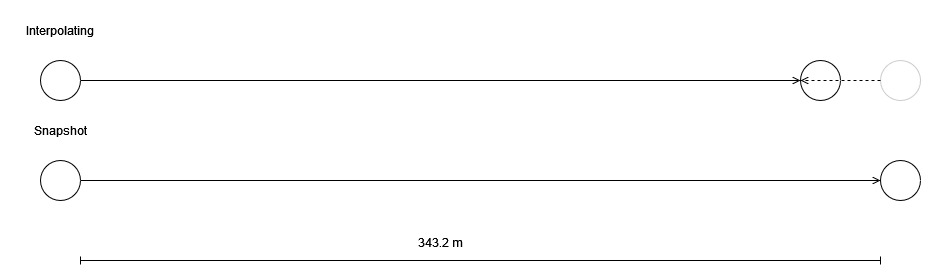
\includegraphics[width=\linewidth]{images/snapshot_explain.jpg}
    \caption{Difference between ray travelling distance using the newly developed interpolating method (top) as opposed to the snapshot method (bottom). In the interpolated version, the ray only travels part of the distance as the receiver travels the remainder.}
\end{figure}
The major downside of this snapshot approach is that it tends to introduce errors when objects or receivers move at high speeds.
As a simple example case, take the scene described in~\ref{im:SnapshotExplain}:
A receiver starts 343 meters away from an emitter and moves towards it at 1/9th the speed of sound, roughly 38 meters per second
(137.2 kilometers per hour, a speed most modern cars can reach without problems).
\newline
Using the snapshot approach, a ray traveling directly from emitter to receiver would arrive after travelling the full 343 meters,
taking 1 second for it to arrive at the receiver.
In actuality, in the time the ray takes to travel the first 90\% of that distance,
the receiver has already travelled the remaining 10\%, making for a response time of 0.9 seconds rather than 1 second.
\newline
To avoid this issue, new intersection logic that takes objects' movements into account is needed.
This check becomes more complicated than its static counterpart as the equation describing the object still needs to be resolved for \(t\),
but now \(t\) is also part of the equation itself.
In this chapter, equations are established and solved to perform intersection checks with moving spheres and surfaces,
as those two should already be sufficient to simulate most scenes.
Resolution for other primitives, such as quadric surfaces, should be derivable using a similar method.
\newline
The general scheme for this is as follows:
First, the object is modelled in a way where its position (or other parameters) is also a function of \(t\).
Then, like with a normal check, the function modelling the ray is injected into this equation,
then resolved.
This will, in the examples below, result in a polynomial function of a higher degree
(2nd and 3rd for spheres and surfaces, respectively), which can then be resolved.
\newline
Unlike with most ray tracing implementations, the magnitude of the ray's direction vector \(v\) becomes significant:
Since the movement of objects checked for intersections is also dependent on time,
objects and the ray must move at the same time scale.
\(v\) must accordingly be scaled to fit the velocity of the ray and the implementation's scale for \(t\) and coordinates.
Otherwise, the intersection calculation will yield incorrect results as at the resulting intersection times,
the ray will either not have travelled to the resulting intersection point yet or will have already surpassed it.
\newline
Note that since the resulting polynomial will be of at least 2nd degree, it can have multiple roots.
Only roots greater than \(t_0\) are relevant as others would represent intersections from before the ray is even launched.
Different primitives might also require different checks to filter out invalid roots depending on how they are modelled,
such as the check for whether a point is inside a triangle described above.
Of the remaining roots, the first one represents the actual intersection time,
the remaining ones can be discarded as they'd only take place if the ray didn't bounce off the first intersection already.

\section{Intersection Checks for Spheres}

A sphere \(C\) is modelled as having a radius \(r\) and a collection of keyframes \(k_n\), each with a center point \(c_{k_n}\) and a time \(t_{k_n}\).
Intersection calculations need to be run separately for each set of consecutive keyframes \(k_1\) and \(k_2\).
\newline
% TODO image
The center point \(c_t\) of \(C\) at time \(t\) can be defined
as a blend between the two keyframes' center points \(c_{k_1}\) and \(c_{k_2}\):

\begin{equation}
    c_t = m \cdot c_{k_1} + (1-m) \cdot c_{k_2}
\end{equation}

\(m\) represents the proportion of \(c_{k_1}\) as opposed to \(c_{k_2}\) at a given time.
The definition of \(m\) depends on the interpolation mode.
For the scope of this thesis, linear interpolation is used, leading to \(m\) being defined as

\begin{equation}\label{MDef}
    m = \frac{t_{k_2} - t}{\Delta t}
\end{equation}

with

\begin{equation}
    \Delta t = t_{k_2} - t_{k_1}
\end{equation}

For non-linear interpolation modes between two keyframes (such as using a sinusoidal function),
\(m\) is defined differently. The math below is still the same until~\eqref{SphereBeforeM} where \(m\) is resolved,
at which point the new definition of \(m\) must be substituted instead of the definition above.
Resolving from there should be trivial, depending on the definition of \(m\).
\newline
For interpolation modes that work with more than two keyframes (such as splines),
\(c_t\) would instead need to be defined using that other interpolation function,
and the scope of which set of keyframes applies to which range of \(t\) would need to be limited accordingly.
Exploring this is outside the scope of this thesis.
\newline

For any given time \(t\),
the surface of \(C\) is then defined as all points \(p\) where the distance to \(c_t\) is the sphere's radius:

\begin{equation}\label{SphereDef}
    \|p-c_t\|^2 = r^2
\end{equation}

Injecting the ray equation~\eqref{RayEq} in place of \(p\) in~\eqref{SphereDef}:

\begin{equation}
    \|P + (t - t_0) \cdot v - c_t\|^2 = r^2
\end{equation}

The squared norm of a vector can be replaced with its dot product with itself (\(\|v\|^2 = v \cdot v \)).
This will allow for the equation to be resolved into a sum of multiple dot products.

\begin{equation*}
    (P - c_{k_2} + t \cdot v - t_0 \cdot v + m \cdot (c_{k_2} - c_{k_1})) \cdot (P - c_{k_2} + t \cdot v - t_0 \cdot v + m \cdot (c_{k_2} - c_{k_1})) = r^2
\end{equation*}

As vector addition inside dot products is distributive (i.e.\ \((a + b) \cdot c = a \cdot c + b \cdot c\)),
this dot product can be resolved into a sum of several dot products,
the factors of which don't require further calculations.
In order to get the equation's shape closer to that of a polynomial,
the fact that scalar multiplication is distributive over addition can be used
to factor out \(t\) and \(m\) from each summand,
then group factors that involve the \(t\) and \(m\) to the same degree.
Defining \(\Delta c = c_{k_2} - c_{k_1}\) for simplicity, this results in a function of \(t\) and \(m\):

\begin{equation}\label{SphereBeforeM}
    \begin{split}
        \|P - c_{k_2}\|^2
        - 2 \cdot t_0 \cdot P \cdot v
        + 2 \cdot t_0 \cdot c_{k_2} \cdot v
        + t_0^2 \cdot \|v\|^2
        - r^2
        \\
        + t \cdot 2 \cdot (P \cdot v - c_{k_2} \cdot v - t_0 \cdot \|v\|^2)
        + m \cdot 2 \cdot (P \cdot \Delta c - c_{k_2} \cdot \Delta c - t_0 \cdot v \cdot \Delta c)
        \\
        + t \cdot m \cdot 2 \cdot v \cdot \Delta c
        + t^2 \cdot \|v\|^2
        + m^2 \cdot \|\Delta c\|^2
        \\
        = 0
    \end{split}
\end{equation}

Now, to get a polynomial function of \(t\), \(m\) needs to be resolved.
The equation for variations of this logic that use different interpolation modes will diverge from here on out,
but should be trivially solvable depending on the definition of \(m\).
Replacing \(m\) with its definition from~\eqref{MDef} for linear interpolation yields the following equation:

\begin{equation*}
    \begin{split}
        \|P - c_{k_2}\|^2
        - 2 \cdot t_0 \cdot P \cdot v
        + 2 \cdot t_0 \cdot c_{k_2} \cdot v
        + t_0^2 \cdot \|v\|^2
        - r^2
        \\
        + t \cdot 2 \cdot (P \cdot v - c_{k_2} \cdot v - t_0 \cdot \|v\|^2)
        + \frac{(t_{k_2} - t) \cdot
            2 \cdot (P \cdot \Delta c - c_{k_2} \cdot \Delta c - t_0 \cdot v \cdot \Delta c)
        }{\Delta t}
        \\
        + \frac{t \cdot (t_{k_2} - t) \cdot 2 \cdot v \cdot \Delta c}{\Delta t}
        + t^2 \cdot \|v\|^2
        + \frac{{(t_{k_2} - t)}^2 \cdot \|\Delta c\|^2}{\Delta t^2}
        \\
        = 0
    \end{split}
\end{equation*}

The partials of the equation created from \(m\) can now be resolved into individual parts with different polynomial degrees.
The resulting summands can then be grouped by their degree to create a polynomial

\begin{equation}\label{SpherePoly}
    d_2t^2 + d_1t + d_0 = 0
\end{equation}

with

\begin{equation}
    d_2 = \|v\|^2 \cdot \Delta t^2
    + \|\Delta c\|^2
    - 2 \cdot v \cdot \Delta c \cdot \Delta t
\end{equation}
\begin{equation}
    d_1 = 2 \cdot (
    (P - c_{k_2}) \cdot v \cdot \Delta t^2
    - t_0 \cdot \|v\|^2
    - (P - c_{k_2} - t_0 \cdot v) \cdot \Delta c \cdot \Delta t
    + t_{k_2} \cdot v \cdot \Delta c \cdot \Delta t
    - t_{k_2} \cdot \|\Delta c\|^2
    )
\end{equation}
\begin{equation}
    \begin{split}
        d_0 = (
        \|P - c_{k_2}\|^2
        + 2 \cdot t_0 \cdot (c_{k_2} - P) \cdot v
        + t_0^2 \cdot \|v\|^2
        ) \cdot \Delta t^2
        \\
        + t_{k_2} \cdot 2 \cdot (P - c_{k_2} - t_0 \cdot v) \cdot dc \cdot \Delta t
        + t_{k_2}^2 \cdot \|dc\|^2
        - r^2 \cdot \Delta t^2
    \end{split}
\end{equation}

If \(r\) also needs to be varied between keyframes,
replace \(r^2\) with the according interpolated value \((m - r_{k_1} + (1-m) r_{k_2})^2\) and resolve accordingly.
\newline
The real roots of~\eqref{SpherePoly} represent all times at which the sphere and ray would theoretically intersect.
Note that all roots \(t\) where \(t < t_{k_1}\) or \(t > t_{k_2}\) must be discarded
because the surface is not described by \(k_1\) and \(k_2\) outside the time frame between them.
Additionally, all roots where \(t \le t_0\) must be discarded as these intersections would happen before the ray is launched,
behind its starting location.
\newline
Of the roots remaining after this filter, the lowest result for \(t\) is the one where the ray and sphere intersect,
assuming the ray does not bounce off of a different object before that.
The coordinates at which the intersection takes place can be calculated by calculating \(R(t)\).

% TODO find case where d2=d1=d0=0

\section{Intersection Checks for Surfaces}

Similarly to spheres, a polygonal surface \(S\) with \(o \ge 3\) corners can also be modelled using a set of keyframes \(k_n\),
each with points \(P_{1..o, k_n}\) for the corners of the surface, with \(o\) being consistent between keyframes.
As with spheres, intersection calculations need to be run separately for each set of consecutive keyframes \(k_1\) and \(k_2\).
\newline
Using \(m\) from~\eqref{MDef} with the same caveats,
each point \(P_{n, t}, 1 \le n \le o\) is calculated as a blend between \(P_{n, 1}\) and \(P_{n, 2}\):

\begin{equation}\label{SurfacePointDef}
    P_{n, t} = m \cdot P_{n, k_1} + (1 - m) \cdot P_{n, k_2}, 1 \le n \le o
\end{equation}

Assuming all points of the polygon are within one surface,
the surface equation from~\eqref{StaticSurface} can be made a function of \(t\)
by replacing \(P_{1..3}\) with their time-dependent counterparts \(P_{1..3, t}\):

\begin{equation}\label{SurfaceDef}
    (p - P_{1, t}) \cdot ((P_{2, t} - P_{1, t}) \times (P_{3, t} - P_{1, t})) = 0
\end{equation}

Injecting~\eqref{RayEq} into~\eqref{SurfaceDef}:

\begin{equation}
    (P + t \cdot v - t_0 \cdot v - P_{1, t}) \cdot ((P_{2, t} - P_{1, t}) \times (P_{3, t} - P_{1, t})) = 0
\end{equation}

The vector cross product is distributive over addition (i.e.\ \( (x + y) \times z = x \times z + y \times z\)),
which can be used to split up the single cross product describing the surface normal into several cross products with single factors,
allowing them to be resolved easier:

\begin{equation*}
    (P + t \cdot v - t_0 \cdot v - P_{1, t}) \cdot
    (P_{2, t} \times P_{3, t} - P_{2, t} \times P_{1, t} - P_{1, t} \times P_{3, t} + P_{1, t} \times P_{1, t})
\end{equation*}

The cross product of a vector with itself is always a vector of zeroes,
which in turn is the identity element for addition (i.e.\ adding it to another vector just results in the other vector),
thus the last of these four cross products (\(P_{1, t} \times P_{1, t}\)) can be discarded:

\begin{equation}\label{SurfaceBeforeCross}
    (P + t \cdot v - t_0 \cdot v - P_{1, t}) \cdot
    (P_{2, t} \times P_{3, t} - P_{2, t} \times P_{1, t} - P_{1, t} \times P_{3, t})
\end{equation}

Each of these cross products should be solved individually before resolving the full equation.
Using~\eqref{SurfacePointDef} to describe a cross product between two generic points \(P_{a, t}\) and \(P_{b, t}\):

\begin{equation}
    P_{a, t} \times P_{b, t}
    = ((1-m) \cdot P_{a, k_2} + m \cdot P_{a, k_1}) \times ((1-m) \cdot P_{b, k_2} + m \cdot P_{b, k_1})
\end{equation}

This can again be simplified by using the fact that the cross product is distributive over addition.
Additionally, scalar factors can be extracted from cross products
as the cross product linearly scales with the individual vectors' magnitude,
so for a scalar \(a\) and two vectors \(x, y\), \(x \times (a \cdot y) = a \cdot (x \times y)\).
This can be exploited to resolve the equation to a polynomial function of \(m\):

\begin{equation}
    \begin{split}
        P_{a, t} \times P_{b, t} =
        P_{a, k_2} \times P_{b, k_2}
        + m \cdot (
        - 2 (P_{a, k_2} \times P_{b, k_2})
        + (P_{a, k_1} \times P_{b, k_2})
        + (P_{a, k_2} \times P_{b, k_1})
        )
        \\
        + m^2 \cdot (
        (P_{a, k_2} \times P_{b, k_2})
        - (P_{a, k_1} \times P_{b, k_2})
        - (P_{a, k_2} \times P_{b, k_1})
        + (P_{a, k_1} \times P_{b, k_1})
        )
    \end{split}
\end{equation}

As with~\eqref{SphereBeforeM}, to get a function of \(t\),
\(m\) needs to replaced with its definition (\eqref{MDef} in this case):

\begin{multline*}
    P_{a, t} \times P_{b, t} =
    \\
    P_{a, k_2} \times P_{b, k_2}
    + \frac{(t_{k_2} - t) \cdot (
        - 2 (P_{a, k_2} \times P_{b, k_2})
        + (P_{a, k_1} \times P_{b, k_2})
        + (P_{a, k_2} \times P_{b, k_1})
        )}{\Delta t}
    \\
    + \frac{{(t_{k_2} - t)}^2 \cdot (
        (P_{a, k_2} \times P_{b, k_2})
        - (P_{a, k_1} \times P_{b, k_2})
        - (P_{a, k_2} \times P_{b, k_1})
        + (P_{a, k_1} \times P_{b, k_1})
        )}{\Delta t^2}
\end{multline*}

Using the distributive law and the binomial theorem,
This can be resolved to a second-degree polynomial

\begin{equation}\label{SurfaceCrossPoly}
    P_{a, t} \times P_{b, t} = f_{2, a, b}t^2 + f_{1, a, b}t + f_{0, a, b}
\end{equation}

with

\begin{equation}\label{SurfaceFStart}
    f_{2, a, b} = (P_{a, k_2} \times P_{b, k_2})
    - (P_{a, k_1} \times P_{b, k_2})
    - (P_{a, k_2} \times P_{b, k_1})
    + (P_{a, k_1} \times P_{b, k_1})
\end{equation}
\begin{equation}
    \begin{split}
        f_{1, a, b} = - \Delta t \cdot (
        - 2 (P_{a, k_2} \times P_{b, k_2})
        + (P_{a, k_1} \times P_{b, k_2})
        + (P_{a, k_2} \times P_{b, k_1})
        )
        \\
        - 2 \cdot t_{k_2} \cdot (
        (P_{a, k_2} \times P_{b, k_2})
        - (P_{a, k_1} \times P_{b, k_2})
        - (P_{a, k_2} \times P_{b, k_1})
        + (P_{a, k_1} \times P_{b, k_1})
        )
    \end{split}
\end{equation}
\begin{equation}\label{SurfaceFEnd}
    \begin{split}
        f_{0, a, b} = \Delta t^2 \cdot (P_{a, k_2} \times P_{b, k_2})
        \\
        + t_{k_2} \cdot \Delta t \cdot (
        - 2 (P_{a, k_2} \times P_{b, k_2})
        + (P_{a, k_1} \times P_{b, k_2})
        + (P_{a, k_2} \times P_{b, k_1})
        )
        \\
        + t_{k_2}^2 \cdot (
        (P_{a, k_2} \times P_{b, k_2})
        - (P_{a, k_1} \times P_{b, k_2})
        - (P_{a, k_2} \times P_{b, k_1})
        + (P_{a, k_1} \times P_{b, k_1})
        )
    \end{split}
\end{equation}

Replacing the cross products in~\eqref{SurfaceBeforeCross} with the polynomial from~\eqref{SurfaceCrossPoly} yields:

\begin{equation*}
    (P + t \cdot v - t_0 \cdot v - P_{1, t}) \cdot
    (f_{2, 2, 3} t^2 + f_{1, 2, 3} t + f_{0, 2, 3} - f_{2, 2, 1} t^2 - f_{1, 2, 1} t - f_{0, 2, 1} - f_{2, 1, 3} t^2 - f_{1, 1, 3} t - f_{0, 1, 3})
    = 0
\end{equation*}

Injecting~\eqref{SurfacePointDef} for \(P_{1, t}\) and
introducing \(g_n = f_{n, 2, 3} - f_{n, 2, 1} - f_{n, 1, 3}\)
and \(\Delta P_1 = P_{1, k_2} - P_{1, k-1}\) for readability
results in this equation:

\begin{equation}\label{SurfaceAfterCross}
    (
    P + t \cdot v - t_0 \cdot v - P_{1, k_2}
    + \frac{t_{k_2} \Delta P_1}{\Delta t}
    - \frac{t \cdot \Delta P_1}{\Delta t}
    ) \cdot
    (
    t^2 g_2
    + t g_1
    + g_0
    )
    = 0
\end{equation}

Again using the fact that vector dot products are distributive over addition to shape this into a sum of several dot products,
then extracting \(t\) and grouping the individual summands by their polynomial degree,
this can be resolved to a third degree polynomial

\begin{equation}\label{SurfacePolyStart}
    t^3d_3 + t^2d_2 + td_1 + d_0 = 0
\end{equation}

With

\begin{equation}
    d_3 = g_2 \cdot v
    - \frac{g_2 \cdot \Delta P_1}{\Delta t}
\end{equation}
\begin{equation}
    d_2 = g_2 \cdot P
    - t_0 \cdot g_2 \cdot v
    - g_2 \cdot P_{1, k_2}
    + \frac{t_{k_2} \cdot g_2 \cdot \Delta P_1}{\Delta t}
    + g_1 \cdot v
    - \frac{g_1 \cdot \Delta P_1}{\Delta t}
\end{equation}
\begin{equation}
    d_1 = g_1 \cdot P
    - t_0 \cdot g_1 \cdot v
    - g_1 \cdot P_{1, k_2}
    + \frac{t_{k_2} \cdot g_1 \cdot \Delta P_1}{\Delta t}
    + g_0 \cdot v
    - \frac{g_0 \cdot \Delta P_1}{\Delta t}
\end{equation}
\begin{equation}\label{SurfacePolyEnd}
    d_0 = g_0 \cdot P
    - t_0 \cdot g_0 \cdot v
    - g_0 \cdot P_{1, k_2}
    + \frac{t_{k_2} \cdot g_0 \cdot \Delta P_1}{\Delta t}
\end{equation}

This polynomial can then be solved using a general cubic formula such as the one described by Abramowitz and Stegun~\cite{AS48}
or Flocke's Algorithm~\cite{Fl15}.
\newline
As with spheres, the real roots of this equation are all the points in time at which the ray and the surface would meet.
Roots \(t\) where \(t < t_{k_1}\) or \(t > t_{k_2}\), as well as roots where \(t \le t_0\),
must be discarded as explained above.
\newline
For the remaining roots, another check needs to be done
for whether the intersection point \(R(t)\) is actually inside the polygon, and not just on the same surface.
With triangles, this can be easily done using the barycentric coordinates as described above.
\newline
The root with the lowest value that satisfies the above conditions again represents the time where the ray and polygon intersect,
assuming there is no intersection happening before. If no root satisfies these conditions, no intersection happens.

\section{Computational Cost}

To gauge the additional computation cost for interpolated intersection checks as opposed to static ones,
consider the analytical solution for static surface intersection calculations as described in~\eqref{StaticSurfaceIntersect}
and using~\eqref{PolygonNormal}.
\newline
Naively calculating a cross product requires 6 multiplications and 3 subtractions.
The dot product requires just 3 multiplications, as does multiplying a scalar onto a coordinate vector.
This means that to calculate the intersection time for a static surface,
a total of 15 additions/subtractions, 15 multiplications and 1 division is required.
As \(n\) is always the same for a surface, it can be cached,
reducing the cost to only 6 additions/subtractions, 9 multiplications and 1 division.
\newline
For the interpolated surface checks, calculating \(f_{0..2, a, b}\) as per~\eqref{SurfaceFStart} to~\eqref{SurfaceFEnd}
alone already takes 71 additions/subtractions and 124 multiplications.
As \(g_{0..2}\) takes 3 sets of \(f\), it thus requires 213 additions/subtractions and 372 multiplications.
Since \(g_{0..2}\) remains the same for a pair of surface keyframes independently of the incoming ray,
it can be cached for each keyframe pair. The same applies for \(\Delta t\) and \(\Delta P_1\),
which otherwise would introduce one and three subtractions respectively.
\newline
Then calculating the surface intersection as per~\eqref{SurfacePolyStart}-\eqref{SurfacePolyEnd}
requires 14 additions/subtractions, 42 multiplications and 3 divisions,
assuming that \(g_{0..2} \cdot v\) and \(\frac{g_{0..2} \cdot \Delta P_1}{\Delta t}\)
are only calculated once each and then reused.
\newline
Additionally, this requires resolving the resulting polynomial,
the cost of which is implementation dependent, but also rather high compared to the static check.
As a reference, in the worst case of none of the polynomial's factors being 0,
the Rust library \verb|roots| (as of version 0.0.8) used in the proof-of-concept, requires 13 additions/subtractions,
58 multiplications and 12 divisions, plus trigonometric and square/cube root functions, the computation cost of which
depends on the CPU architecture and cannot be reduced to a number of simple operations.
\newline
In total, the amount of calculations, especially multiplications, to perform balloons up with this more complex method.

\section{Looping Scenes And Full Algorithm}

A full algorithm to check for intersections then needs to traverse every pair
(or set, for interpolation modes working with more than two keyframes) of keyframes
and run the intersection check as described above.
\newline
For a surface, this algorithm looks as follows:

\begin{verbatim}
// define keyframes and ray here
for index in 0..(keyframes.len - 1) {
    k1 = keyframes[index];
    k2 = keyframes[index+1];
    (d3, d2, d1, d0) = polynomial_parameters(k1, k2);
    // get all potential intersections
    roots = solve_cubic_function(d3, d2, d1, d0);
    intersection_time = null;
    for root in roots {
        // filter intersections
        if root < ray.launch_time {
            continue;
        }
        if root < k1.time || root > k2.time {
            continue;
        }
        // potential further checks here

        if intersection_time == null
            || root < intersection_time {
                intersection_time = root
        }
    }
    // no need to check future keyframes
    // if an intersection was found
    if root != null {
        return root;
    }
}
// no intersection
return null;
\end{verbatim}